\documentclass[fr]{../../../eplsummary}

\usepackage{../../../eplmath}
\usepackage{float}

\graphicspath{{img/}}

\newcommand{\Cmn}{\C^{m \times n}}
\newcommand{\Cmm}{\C^{m \times m}}
\newcommand{\Cn}{\C^{n}}
\newcommand{\Cm}{\C^{m}}
\newcommand{\frob}[1]{\norm{#1}_{\textnormal{F}}}

\DeclareMathOperator{\nullspace}{null}
\DeclareMathOperator{\range}{range}
\DeclareMathOperator{\rank}{rank}
\DeclarePairedDelimiterX{\inp}[2]{\langle}{\rangle}{#1, #2}
\DeclareMathOperator{\tr}{tr}

\hypertitle[']{Analyse numérique}{5}{INMA}{1170}
{Gilles Peiffer}
{François Henrotte et Jean-François Remacle}

%TODO annexe Gmsh (cm 2)?

\section{Bases d'algèbre linéaire}
L'algèbre linéaire est l'étude de l'équation
\[
Ax = b\,.
\]
Il y a quatre façons de voir cette équation:
\begin{enumerate}
	\item Comme un \emph{produit matrice-vecteur}, où
	\[
	A \in \Cmn\,, \quad x \in \Cn\,, \quad b \in \Cn\,.
	\]
	\item Comme une \emph{expression tensorielle}:
	\[
	b_i = \sum_{j=1}^{n} a_{ij}x_i\,,
	\]
	où $a_{ij}$ est l'entrée
	à la $i$\ieme{} ligne
	et la $j$\ieme{} colonne de $A$.
	\item Comme disant que
	\emph{$b$ est dans le \textbf{column space} de $A$}\footnote{Espace vectoriel sous-tendu par les colonnes de $A$.},
	et est donc une combinaison linéaire des colonnes de $A$.
	\[
	b = Ax = \sum_{j=1}^{n} x_j a_j\,,
	\]
	où $a_j$ est la $j$\ieme{} colonne de $A$.
	\item Comme une \emph{application linéaire} de $\Cn$ dans $\Cm$:
	\begin{align*}
	A \colon \Cn &\to \Cm\,,\\
	x &\mapsto Ax\,.
	\end{align*}
	On a donc les propriétés suivantes:
	\[
	\begin{array}{rcl@{\quad}l}
		A(x+y) & = & A(x) + A(y)\,, & \quad \forall x,y \in \Cn\,,\\
		A(\alpha x) & = & \alpha A(x)\,, & \quad \forall x \in \Cn\,,
		\quad \alpha \in \C\,.
	\end{array}
	\]
\end{enumerate}

\subsection{Produit matrice-matrice}
Le produit matrice-matrice
\[
B = AC\,, \quad B \in \C^{\ell \times n}\,,\quad A \in \C^{\ell \times m}\,,\quad C \in \Cmn
\]
est une généralisation du produit matrice-vecteur vu précédemment.
On peut également l'écrire
\begin{align*}
	b_{ij} &= \sum_{k=1}^{m} a_{ik}c_{kj}\,.
\end{align*}
Chaque colonne de $B$ est une combinaison linéaire
des colonnes de $A$.

\subsection{Définitions}
\begin{mydef}[Column space]
	Le \emph{column space} d'une matrice $A \in \Cmn$,
	également noté $\range(A)$ est défini comme
	\[
	\range(A) = \mathrm{span}\{a_1, a_2, a_3, \dots, a_n\}\,.
	\]
\end{mydef}
\bigbreak
\begin{mydef}[Kernel]
	Le \emph{kernel} (\emph{noyau}, encore appelé \emph{null space}) d'une matrice $A \in \Cmn$
	est défini comme
	\[
	\nullspace(A) = \set{x \in \Cn \suchthat Ax = 0}\,.
	\]
	Les composantes de chaque vecteur de $\nullspace(A)$
	sont les coefficients d'une combinaison linéaire nulle
	des colonnes de $A$.
	\[
	Ax = 0 \iff \sum_{j=1}^{n} x_j a_j = 0\,.
	\]
\end{mydef}
\bigbreak
\begin{mydef}[Rang]
	Le \emph{rang} d'une matrice $A \in \Cmn$
	est défini comme la dimension de $\range(A)$:
	\[
	\rank(A) = \dim(\range(A))\,.
	\]
	Les espaces vectoriels sous-tendus
	par les lignes et les colonnes d'une matrice (carrée ou rectangulaire)
	ont toujours la même dimension.
	On appelle rang de la matrice $A$ cette dimension.
	On a donc nécessairement
	\[
	\rank(A) \le \min(m,n)\,.
	\]

	On dit qu'une matrice est \emph{de plein rang} lorsque
	\[
	\rank(A) = \min(m,n)\,.
	\]
	Une matrice est de plein rang si et seulement si
	jamais deux vecteurs différents de son domaine n'ont la même image.
	Cela implique que l'application
	\[
	A \colon \Cn \to \range(A) \subseteq \Cm
	\]
	est bijective\footnote{La démonstration est en page 7 du livre.}.
	% TODO add bib reference, maybe put this in an appendix?

	Il n'y a qu'une seule matrice \emph{de rang zéro} par dimension:
	la matrice nulle.

	Pour ce qui en est des matrices \emph{de rang un},
	prenons les vecteurs suivants:
	\begin{align*}
		u &\in \C^{m \times 1}\,,\\
		v &\in \C^{1 \times n}\,.
	\end{align*}
	Leur produit s'écrit
	\[
	\big(uv\big)_{ij} = u_i v_j\,.
	\]
	Cette matrice $\big(uv\big)_{ij}$ est de rang un,
	car toutes ses colonnes sont multiples de $u$.
\end{mydef}
\bigbreak
\begin{mydef}[Matrice inversible]
	Une matrice carrée $A \in \Cmm$ est \emph{inversible}
	si elle satisfait les propositions ci-dessous.
	Toutes les propositions suivantes sont équivalentes:
	\begin{enumerate}[label=(\alph*)]
		\item $A$ est inversible;
		\item $\rank(A) = m$ ($A$ est de plein rang);
		\item $\range(A) = \Cm$;
		\item $\nullspace(A) = \{0\}$ (et \emph{non pas} $\emptyset$);
		\item $0$ n'est pas une valeur propre de $A$;
		\item $0$ n'est pas une valeur singulière de $A$;
		\item $\det(A) \ne 0$.
	\end{enumerate}
\end{mydef}
\bigbreak
\begin{mydef}[Matrice adjointe]
	Si $A \in \Cmn$, la \emph{matrice adjointe} de $A$,
	notée\footnote{Une autre notation possible est $A^{\dag}$.} $A^*$,
	est la matrice obtenue:
	\begin{itemize}
		\item en prenant le complexe conjugué de chaque coefficient;
		\item en permutant lignes et colonnes.
	\end{itemize}
	Remarquons que si $A$ est réelle, $A^* = A^T$.
\end{mydef}
\subsection{Produit scalaire}
Un \emph{produit scalaire} (ou \emph{produit intérieur})
est une opération bilinéaire
\[
\inp{\cdot}{\cdot} \colon \Cm \times \Cm \to \C
\]
telle que
\[
x^* y = \sum_{i=1}^{m} \widebar{x}_i y_i\,,
\]
où $\widebar{x}_i$ est l'entrée $i$ du complexe conjugué de $x$.

Reprenons nos vecteurs $u \in \C^{1 \times m}$
et $v \in \C^{m \times 1}$.
On a que
\[
uv = \sum_{i=1}^{m} u_i v_i\,.
\]
Comme l'opération est bilinéaire,
on a
\[
\renewcommand{\arraystretch}{1.5}
\begin{array}{rcl@{\quad}l}
	\big(x_1 + x_2\big)^* y & = & x_1^* y + x_2^* y\,, & \forall x_1, x_2, y \in \Cm\,,\\
	x^* \big(y_1 + y_2\big) & = & x^* y_1 + x^* y_2\,, & \forall x, y_1, y_2 \in \Cm\,,\\
	\big(ax\big)^* by & = & \widebar{a}b x^* y\,, & \forall a,b \in \C\,, \quad \forall x,y \in \Cm\,.
\end{array}
\]
\subsubsection{Longueur d'un vecteur}
Avec ce produit scalaire,
il est possible de définir la longueur d'un vecteur:
\[
\norm{x} = \sqrt{x^* x}\,, \quad \textnormal{si } x\in \R^{m}\,.
\]

\subsubsection{Angle entre deux vecteurs}
Le produit scalaire permet aussi
de définir l'angle entre deux vecteurs:
\[
\cos \alpha = \frac{x^* y}{\norm{x}\norm{y}}\,.
\]
\subsubsection{Orthogonalité}
Grâce au produit scalaire,
on peut définir le concept d'orthogonalité
\begin{itemize}
	\item de deux vecteurs:
	\[
	x^* y = 0 \iff y^* x = 0\,,
	\]
	\item d'un ensemble $\mathcal{S}$ de vecteurs:
	\[
	x^* y = 0\,, \quad \forall x,y \in \mathcal{S} \suchthat x \ne y \implies \textnormal{ils sont linéairement indépendants,}
	\]
	\item de deux ensembles $\mathcal{S}$ et $\mathcal{S}'$
	de vecteurs non nuls:
	\[
	x^* y = 0\,,\quad \forall x \in \mathcal{S}\,,\quad \forall y \in \mathcal{S}'\,.
	\]
\end{itemize}
\subsubsection{Décomposition orthogonale}
Soit un ensemble $\mathcal{Q} = \{q_1,q_2,\dots,q_n\}$ de vecteurs orthonormés
formant une base orthonormée
pour un sous-espace de dimension $n \le m$ de $\Cm$.
On a alors\footnote{Où $\delta_{ij}$ est le \emph{symbole de Kronecker}.}
\[
q_i^* q_j = \delta_{ij}\,,\quad i,j = 1,\dots,n\,.
\]
Soit $v \in \Cm$.
On a la décomposition orthogonale
\begin{align*}
v &= r + \sum_{i=1}^{n} q_i^* v q_i\\
&= r + \sum_{i=1}^{n} q_i q_i^* v\,,
\end{align*}
avec $q_i^* r = 0$,
c'est-à-dire $r \perp \mathcal{Q}$.
\subsubsection{Matrice unitaire}
Une matrice unitaire est une matrice carrée vérifiant
\[
Q^* = Q^{-1} \iff Q^* Q = I\,,
\]
qui s'écrit également
\[
q_1^* q_2 = \delta_{ij}\,,
\]
en termes des colonnes de $Q$.
Les colonnes d'une matrice unitaire de $\Cmm$
forment une base orthonormée pour $\Cm$.
\subsubsection{Isométrie}
Une matrice unitaire laisse le produit scalaire invariant:
\[
\big(Qx\big)^* Qy = x^* y\,.
\]
Les longueurs des vecteurs et les angles qu'ils forment
sont donc également invariants\footnote{En mécanique des solides déformables,
cela donne lieu aux rotations et aux réflexions
selon que $\det(Q)$ soit $1$ ou $-1$ respectivement.}.
\subsection{Norme vectorielle}
Une norme vectorielle est une fonction
\[
\norm{\cdot} \colon \Cn \to \R
\]
satisfaisant les trois hypothèses suivantes:
\begin{itemize}
	\item \emph{séparation}: $\norm{x} \ge 0$
	avec l'égalité si et seulement si $x = 0$;
	\item \emph{inégalité triangulaire}: $\norm{x+y} \le \norm{x} + \norm{y}$;
	\item \emph{homogénéité absolue}: $\norm{ax} = \abs{a}\norm{x}\,,\quad \forall a \in \C$.
\end{itemize}

\begin{myrem}
	\emph{Le produit scalaire n'est donc pas une norme},
	car il ne satisfait pas la deuxième hypothèse.
	Cependant, sa racine carrée l'est.
\end{myrem}

Il existe beaucoup de normes différentes,
comme par exemple les $p$-normes (ou $\ell^p$-normes):
\begin{itemize}
	\item la norme $\ell^1$ définie par
	\[
	\norm{x}_1 \coloneqq \sum_i \abs{x_i}\,;
	\]
	\item la norme $\ell^2$ définie par
	\[
	\norm{x}_2 \coloneqq \sqrt{\sum_i x_i^2}\,;
	\]
	\item la norme $\ell^p$ définie par
	\[
	\norm{x}_p \coloneqq \left(\sum_i \abs{x_i}^p\right)^{1/p}\,;
	\]
	\item la norme $\ell^{\infty}$ définie par
	\[
	\norm{x}_\infty \coloneqq \max_i \abs{x_i}\,.
	\]
\end{itemize}
On peut donner une représentation graphique de ces normes vectorielles.
On définit pour cela les \emph{boules unitaires} (\emph{unit balls}):
\[
B_p^m = \set[\big]{x \in \Cm \suchthat \norm{x}_p \le 1}\,.
\]
\begin{figure}[H]
	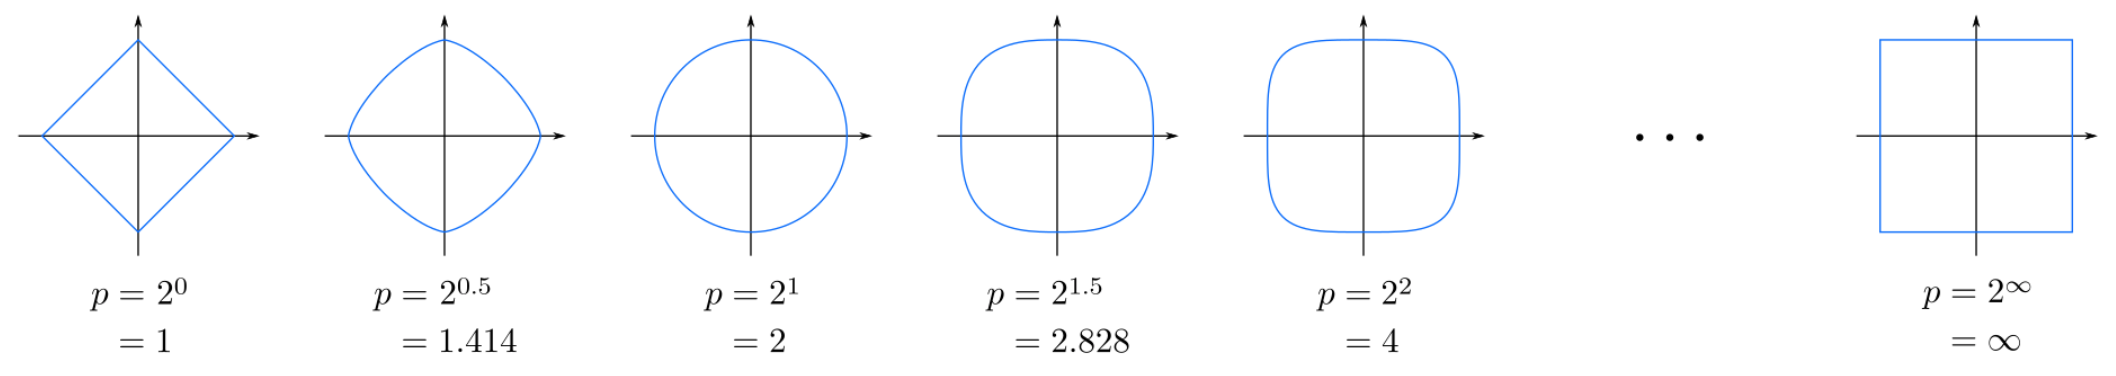
\includegraphics[width=\textwidth]{unit_balls.png}
	\caption{Une visualisation des boules $B_p^1$ pour $p \in \intervalco{1}{+\infty}$.}
	\label{fig:unit_balls}
	% TODO bib ref (wikipedia; unit ball)
\end{figure}
Comme on le voit sur la figure,
\[
B_p^m \subsetneq B_q^m\,,\quad \forall p < q\,.
\]
\subsection{Norme matricielle}
La norme matricielle induite par une norme vectorielle
est une norme pour les matrices
regardées comme des opérateurs sur les vecteurs.
Soit $A \in \Cmn$ un opérateur $A \colon \Cn \to \Cm$
et $\norm{\cdot}_{(m)}$ et $\norm{\cdot}_{(n)}$ deux normes vectorielles
respectivement sur $\Cm$ et $\Cn$.
On définit la norme matricielle $\norm{\cdot}_{(m,n)}$
induite par ces normes vectorielles par
\[
\norm{A}_{(m,n)} \coloneqq \sup_{x \in \Cn \setminus \{0\}} \frac{\norm{Ax}_{(m)}}{\norm{x}_{(n)}}\,.
\]
Comme toute norme doit satisfaire l'hypothèse d'homogénéité absolue,
et que $A$ est linéaire,
on voit que la norme de $x$ n'intervient pas dans la norme matricielle.
On peut également définir cette norme sans division:
\[
\norm{A}_{(m,n)} \coloneqq \sup_{x \in B_p^m} \norm{Ax}_{(m)}\,.
\]
On a l'égalité pratique suivante:
\[
\norm{A}_{(m, n)} \ge \frac{\norm{Ax}_{(m)}}{\norm{x}_{n}}\,.
\]

\subsubsection{$\norm{A}_1$}
\label{sec:1-norm}
% TODO cite example 3.3 in book
Soit la 1-norme matricielle $\norm{\cdot}_1$
induite par les normes vectorielles
$\norm{\cdot}_{(m)} = 1$ et $\norm{\cdot}_{(n)} = 1$.
Soit $A \in \Cmn$.
On prend $x \in B_{1}^{n}$,
et on écrit (où $a_j$ est la $j$\ieme{} colonne de $A$)
\begin{align*}
\norm{Ax}_1 &= \norm{\sum_{j=1}^{n} x_j a_j}_1 \\
&\le \sum_{j=1}^{n} \abs{x_j} \norm{a_j}_1 \\
&\le \max_{1 \le j \le n} \norm{a_j}_1\,.
\end{align*}
On en déduit que
\[
\norm{A}_1 \le \max_{1 \le j \le n} \norm{a_j}_1\,.
\]
Si on choisit $x = e_j$,
où $j$ maximise $\norm{a_j}_1$,
on atteint cette borne,
et donc la norme matricielle est
\[
\norm{A}_1 = \max_{1 \le j \le n} \norm{a_j}_1\,.
\]

\subsubsection{$\norm{A}_{\infty}$}
% TODO cite example 3.4 in book
Soit $A \in \Cmn$.
On prend $x \in B_{\infty}^{n} \implies \abs{x_j} \le 1 \quad \forall j$.
\begin{align*}
	\norm{Ax}_{\infty} &= \norm{\sum_{j=1}^{n} x_j a_j}_{\infty} \\
	&= \sum_{j=1}^{n} \norm{x_j a_j}_{\infty} \\
	&\le \sum_{j=1}^{n} \abs{x_j} \norm{a_j}_{\infty} \\
	&= \sum_{j=1}^{n} \abs{x_j} \max_{1 \le i \le m} a_{ij} \\
	&\le \sum_{j=1}^{n} \max_{1 \le i \le m} a_{ij} \\
	&= \max_{1 \le i \le m} \sum_{j=1}^{n} \abs{a_{j}} \\
	&= \max_{1 \le i \le m} \norm{a_i^*}_1\,.
\end{align*}
On applique le même raisonnement qu'à la \sectionref{1-norm}
pour trouver que la borne est serrée:
\[
\norm{A}_{\infty} = \max_{1 \le i \le m} \norm{a_i^*}_1\,.
\]

\subsubsection{Borner \norm{AB}}
Soient $\norm{\cdot}_{(\ell)}$,
$\norm{\cdot}_{(m)}$ et $\norm{\cdot}_{(n)}$
des $p$-normes vectorielles pour $\C^{\ell}$, $\Cm$ et $\Cn$ respectivement.
Soient $A \in \C^{\ell \times m}$ et $B \in \Cmn$.
On sait que
\begin{align*}
\norm{ABx}_{\ell} &\le \norm{A}_{(\ell, m)} \norm{Bx}_{(m)}\\
&\le \norm{A}_{(\ell, m)} \norm{B}_{(m, n)} \norm{x}_{(n)}\,.
\end{align*}
On trouve alors
\[
\norm{AB}_{\ell, n} \le \norm{A}_{(\ell, m)} \norm{B}_{(m, n)}\,.
\]
Notons qu'en général, cette inégalité n'est pas serrée.

\subsection{Inégalités de Cauchy-Schwarz et de Hölder}
Calculer les $p$-normes matricielles avec $p \ne 1, \infty$ est compliqué,
et afin de résoudre ce problème,
on note que les produits intérieurs peuvent être bornés
en utilisant des $p$-normes.
Soient $p$ et $q$ tels que
\[
\frac{1}{p} + \frac{1}{q} = 1\,, \quad 1 \le p, q \le \infty\,.
\]
L'\emph{inégalité de Hölder} dit alors que,
pour tout vecteurs $x$ et $y$,
\[
\abs{x^* y} \le \norm{x}_p \norm{y}_q\,.
\]
Dans le cas particulier $p = q = 2$,
on a l'\emph{inégalité de Cauchy-Schwarz}:
\[
\abs{x^* y} \le \norm{x}_2 \norm{y}_2\,.
\]
Ces deux bornes sont serrées.

\begin{myrem}
	Deux remarques sont à faire ici:
	\begin{itemize}
		\item Il ne faut pas confondre cette inégalité
		avec l'inégalité triangulaire qui implique une somme.
		\item Cette inégalité n'est valable que pour certaines normes.
	\end{itemize}
\end{myrem}

\subsection{Norme de Frobenius}
La norme de Frobenius\footnote{Également appelée norme de Hilbert-Schmidt.} d'une matrice
n'est pas induite par une norme vectorielle.
Pour être une norme matricielle,
il suffit que la norme vérifie les trois propriétés des normes vectorielles,
appliquées dans l'espace vectoriel des matrices, de dimension $mn$.
La norme de Frobenius est définie comme
\begin{align*}
\frob{A} &= \left(\sum_{i=1}^{m} \sum_{j=1}^{n} \abs{a_{ij}^2}\right)^{1/2} \\
&= \left(\sum_{j=1}^{n} \norm{a_{j}}_2 \right)^{1/2} \\
&= \sqrt{\tr(A^* A)}\,.
\end{align*}

\begin{mytheo}[Invariance sous multiplication unitaire]
La norme de Frobenius et la $2$-norme matricielle sont invariantes
sous multiplication par une matrice unitaire,
c'est-à-dire que pour tout $A \in \Cmn$, et $Q \in \Cmm$ unitaire,
on a
\[
\norm{QA}_2 = \norm{A}_2 \quad \textnormal{et} \quad \frob{QA} = \frob{A}\,.
\]
\end{mytheo}

La norme de Frobenius peut être utilisée pour borner un produit de matrices.
Posons $C = AB$ avec $C \in \C^{n \times m}$
dont les entrées sont les $c_{ik} = a_i^* b_j$.
Par l'inégalité de Cauchy-Schwarz,
on a alors $\abs{c_{ij}} \le \norm{a_i}_2 \norm{b_j}_2$.
En mettant au carré des deux cotés et en sommant, on trouve
\begin{align*}
	\frob{C}^2 = \frob{AB}^2 &= \sum_{i=1}^{n} \sum_{j=1}^{m} \abs{c_{ij}^2} \\
	&\le \sum_{i=1}^{n} \sum_{j=1}^{m} \left(\norm{a_i}_2 \norm{b_j}_2 \right)^2 \\
	&= \sum_{i=1}^{n} \left( \norm{a_i}_2 \right)^2 \sum_{j=1}^{m} \left( \norm{b_j}_2 \right)^2 \\
	&= \frob{A}^2 \frob{B}^2\,.
\end{align*}

\end{document}
